\section{Optimization Summary}

\begin{center}
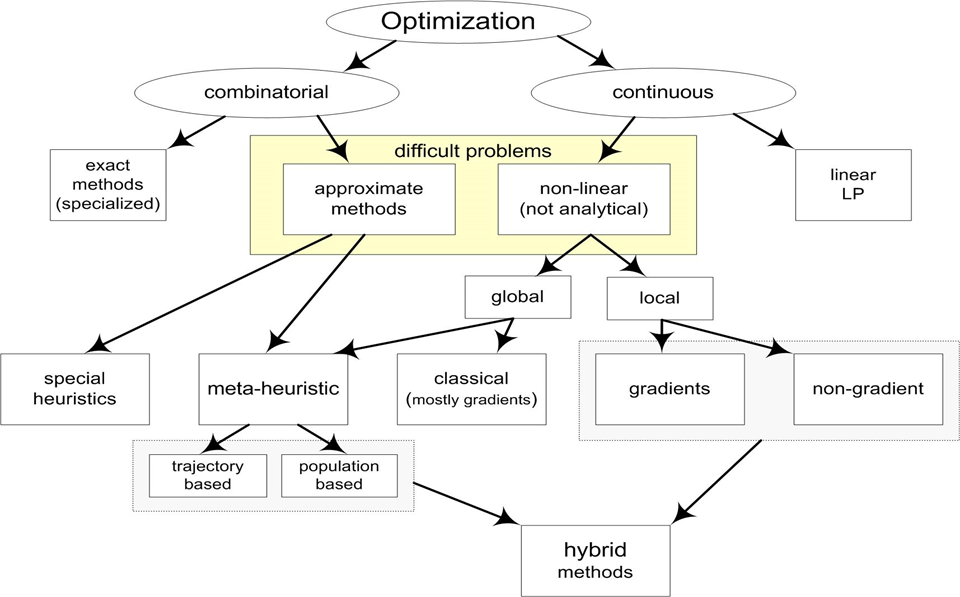
\includegraphics[width=0.7\textwidth]{./Content/OptimizationSummary/Summary}
\end{center}

\textbf{Auswahlhilfe für Algorithmen:}
  \begin{itemize}
    \item Kontinuierliche Lineare Probleme: Lineare Programmierung, Integer Programmierung
    \item Kontinuierliche nichtlineare Probleme: Gradientenverfahren (Steepest Descent, Newton) oder bei komplexeren Problemen Heuristiken (Ant Colony oder Genetische Algorithmen)
    \item Einfache/gutartige Probleme: Trajektorienbasierte Algorithmen (Hill-Climbing, Tabu Search, Simulated Annealing)
    \item Komplexe Kombinatorische Probleme: Ant Colony oder Genetische Algorithmen
    \item Komplexe Parameteroptimierungen: Particle Swarm Optimization oder Genetische Algorithmen
  \end{itemize}

